\documentclass[11pt,a4paper]{article}
\usepackage[T1]{fontenc}
\usepackage[utf8]{inputenc}
\usepackage[margin=22mm]{geometry}
\usepackage{booktabs,longtable,tabularx,array,graphicx,pdfpages}
\usepackage{xcolor}
\usepackage[hidelinks]{hyperref}
\setlength{\parindent}{0pt}
\setlength{\parskip}{6pt}
\renewcommand{\arraystretch}{1.18}
\newcommand{\pending}{\textit{Pending actual records}}
\title{RIVR -- Texas Hold'em\\Iteration Planning, Execution and Testing}
\author{CS 482, Team 23\\Chris, Finn, Kelechi and Royal}
\date{November 3, 2026}
\begin{document}
\maketitle
\textbf{Purpose and provenance.} This document repairs the missing Iteration 1 documentation and records Iteration 2 work. Iteration 1 is reconstructed retrospectively; it is not represented as a report submitted before the original deadline. Team plans were supplied by Chris. Branch commits are contribution evidence; main-branch delivery and professor acceptance are separate checks. Individual reflections, actual hours and acceptance decisions require human confirmation.

The Iteration 2 assignment supplied in chat lists November 5, 2026 as the nominal due date, with instructions to verify Moodle and a Sunday-night grace period. The exact cutoff, release date and presentation time must be verified; the demo is not a delivery extension. Chris reports that the Iteration 2 planning email was sent October 27, 2026 at 7:47 PM local time (America/New\_York). This records the student's reported sent time; professor receipt and acceptance are not inferred.

\setcounter{tocdepth}{1}
{\small\tableofcontents}
\newpage
\section{System Design}
RIVR follows the existing three-layer design: React/TypeScript presentation, Django/REST Framework application services, and PostgreSQL persistence. Session authentication and CSRF protect account writes. Server-owned event IDs, transactions and user-row locks protect XP and chip rewards. Avatar bytes are validated and normalized before storage.

\subsection{Diagrams}
The following sequence diagram models a proposed multiplayer action and hand-completion scenario. It shows invalid-action rollback, authoritative result calculation, transactional XP/trophies and recipient-filtered publication only after commit. The game service, game-action endpoint and Channels transport are planned, not implemented by this modelling deliverable. The progression service and underlying framework/database exist now. A diagram is not evidence of a shipped gameplay engine.

Editable source: \texttt{docs/diagrams/multiplayer-sequence.mmd}. Vector rendering is generated by \texttt{scripts/render\_gameplay\_diagram.py}. The model deliberately distinguishes shared pots from outright wins and keeps private hole cards private.
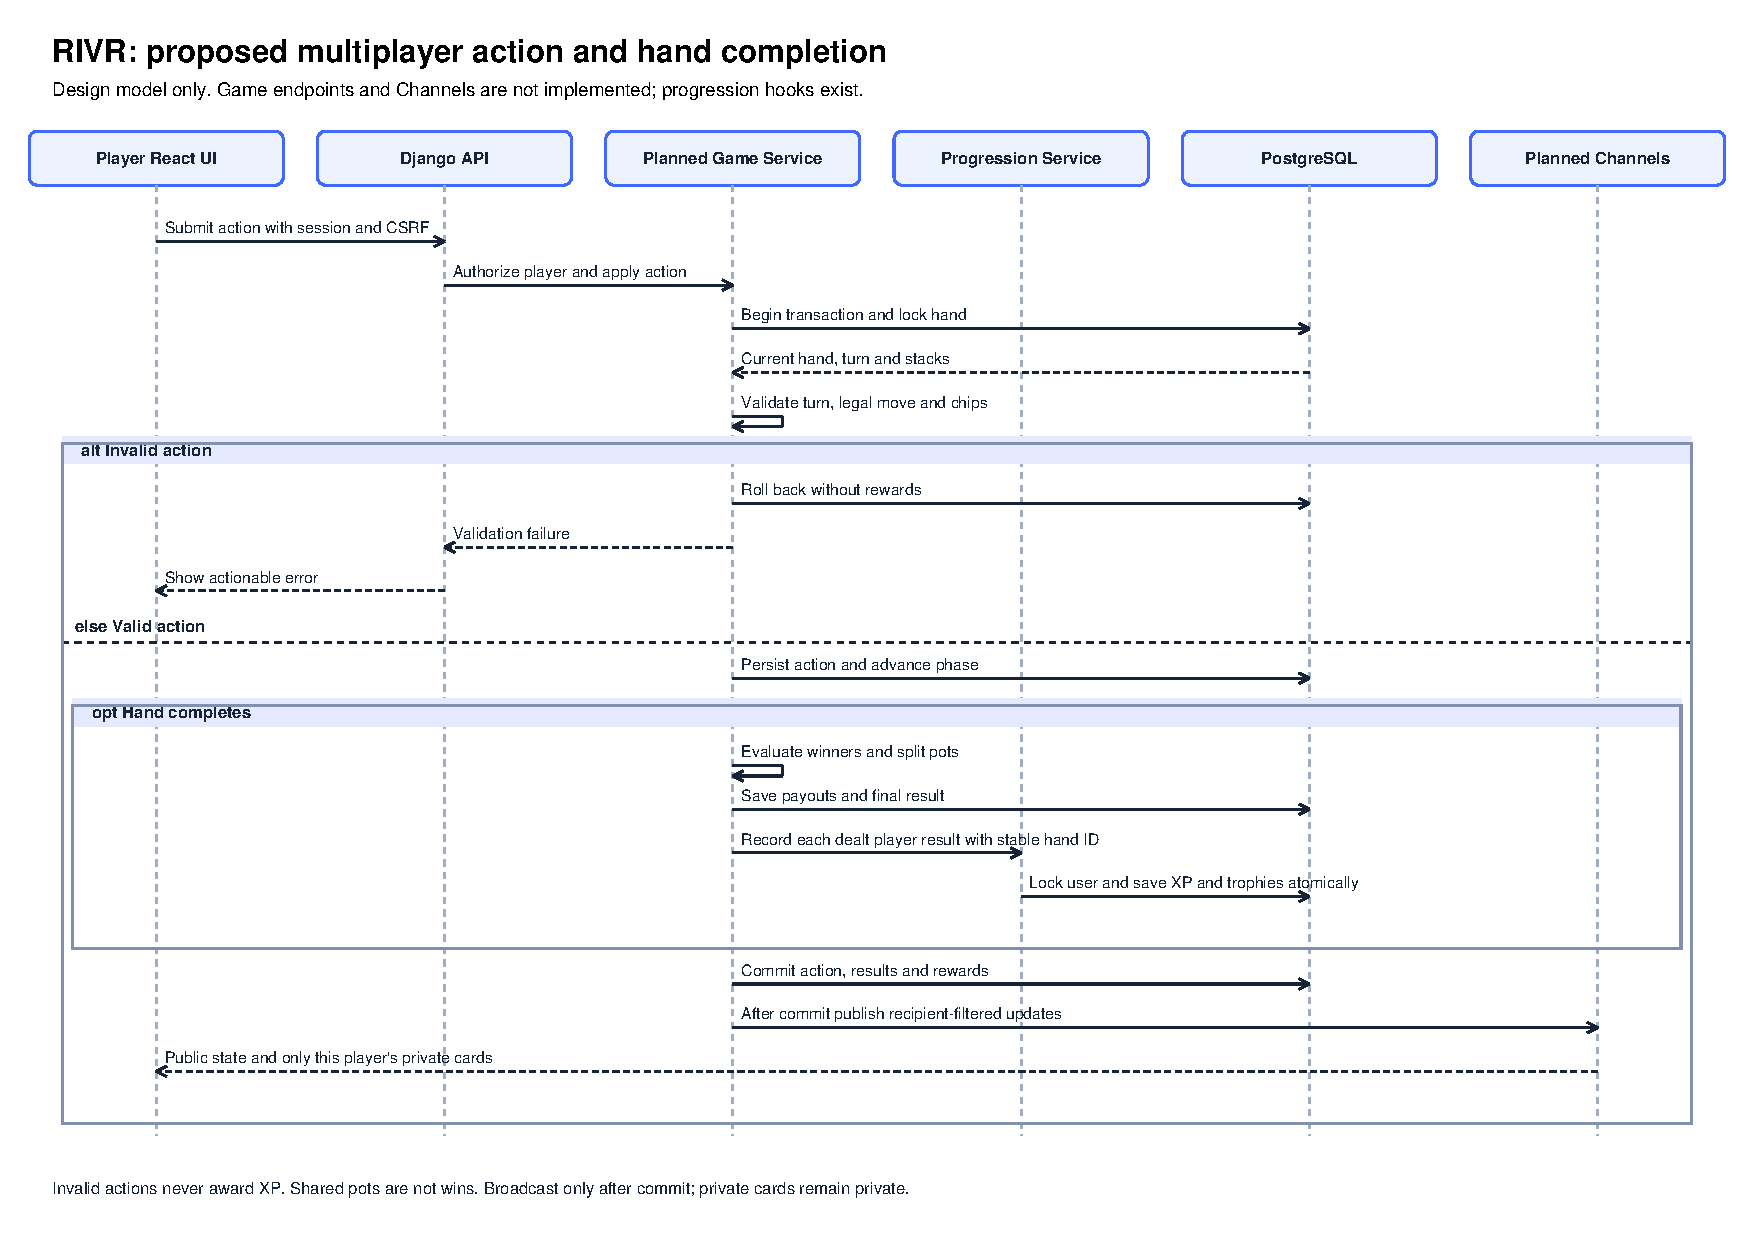
\includepdf[pages=1,fitpaper=true,pagecommand={}]{../diagrams/multiplayer-sequence.pdf}

\section{Main Iteration Planning Table}
\begin{tabularx}{\textwidth}{@{}l l X r@{}}
\toprule Iteration & Owner & Planned stories & Points\\\midrule
1 & Chris & S13 public table; S10 browse tables & 4\\
1 & Finn & S2 registration; S1 login/logout; S4 guests & 4\\
1 & Kelechi & S23 admin cleanup; S35 themes & 4\\
1 & Royal & S5 image upload; S14 starting chips; S29 daily chips & 4\\
\midrule 1 & Team & Updated team plan & 16\\\midrule
2 & Chris & S32 XP/achievements (3); S18 leaderboard (1) & 4\\
2 & Finn & S19 add/remove friends & 5\\
2 & Kelechi & S16 chip balance (2); S15 buy-in (1); S17 stats (1) & 4\\
2 & Royal & S11 filters (1); S27 private table (1); S26 spectate (2) & 4\\
\midrule 2 & Team & Reported planning-email content & 17\\\bottomrule
\end{tabularx}

These are planned points, not accepted points. The original workbook lists S5 as 3 points and S14 as unestimated; Chris supplied an updated Iteration 1 team plan of 2 and 1. Instructor estimate confirmation is not supplied. Planned ownership is distinct from commit authorship. Some S11 filtering and chip-persistence behavior existed earlier; the team must identify incremental work and avoid counting the same delivery twice.

\section{Iteration 1: Planning and Execution}
\subsection{Reported plan}
The original planning window was October 12--22, 2026, with an October 21 internal completion target and an October 22 nominal deadline to confirm on Moodle. Four points were assigned to each teammate, for 16 planned points. The report preserves the updated team plan rather than inventing a prior submission date. Planning-email timing remains \pending.

\subsection{Reconstructed work}
\begin{tabularx}{\textwidth}{@{}l l X@{}}
\toprule Stories & Planned owner & Observed source / original authorship evidence\\\midrule
S13/S10 & Chris & Tables, create/lobby screens and tests; S13 commit \texttt{9b87b7d}.\\
S2/S1/S4 & Finn & Authentication/session and frontend commits \texttt{402f931}, \texttt{03cb335}, \texttt{a8606f1}.\\
S23/S35 & Kelechi & Cleanup/theme commits \texttt{54bae1f}, \texttt{d3e56f2}, \texttt{f0ac4cb}.\\
S5/S14/S29 & Royal assigned & Chris later covered these as requested in this session. \texttt{9b21c1e} is authored by Chris on October 26. It is not attributed to Royal or backdated.\\\bottomrule
\end{tabularx}

All ten feature areas exist in the current code, but this does not prove their presence at the original cutoff. The fetched main tip at the start of this audit was \texttt{7a3d567}, October 26. The October 26 avatar/reward work cannot be claimed as a demonstrated original-deadline delivery. Other teammates' local/unpushed work cannot be established from this clone alone.

Actual hours for each story, instructor acceptance, total accepted points, velocity and historical cycle time: \pending. The original 14--16 hours/person estimate is not an actual time log. The CSV work-log template preserves unknowns as blank, not zero.

\subsection{Testing and reflection}
The professor reported that the committed coverage image covered only two files. That historical S23 report covers cleanup/admin only (61 statements and 12 branches), not the team application. It is retained with an explicit scope correction. Current full-application evidence is supplied separately and does not retroactively cure the original submission.

Proposed process improvements, awaiting individual team confirmation: write the report during the iteration; check every file included in coverage; link real issues in commits; rehearse the real database flow; preserve authorship when merging; and ensure every teammate attends and explains their own work. The professor reported Kelechi presented alone. Attendance explanations belong to the students and must not be manufactured.

\section{Iteration 2: Planning and Execution}
\subsection{Team branches and contributions}
Chris confirmed each member works on their own branch. Fetched branch refs and original commit authors are recorded in \texttt{docs/quality/branch-evidence.json}. Finn's \texttt{feature/S19-friends} includes \texttt{798af8e}, \texttt{09166e7} and \texttt{e3c7733}; it was not in the audited main tip. Kelechi's historical cleanup/theme branches and Chris's \texttt{saia} are visible. A missing or unpushed Royal/current teammate ref is not evidence of non-contribution. The team must provide those refs and integrate reviewed work by the cutoff.

\subsection{Chris: S32 and S18}
\textbf{S32, 3 planned points, issue \#45.} Twenty-four trophies have hidden-until-earned metadata, private account collection access and server-owned rewards. Real avatar upload, public game creation and recorded theme changes award persisted XP. Each trophy unlocks once; Against the Odds pays 50 XP again per distinct qualifying 7--2 offsuit win. Outright hand wins pay 100 XP and tournament wins 1,000 XP per unique result. Awards stack and retries do not pay twice. Splits are not wins.

Gameplay, tournament, friends and messaging trophies have tested trusted hooks and explicit validation rules, but their authoritative feature integrations are not shipped by this work. This is a partial integration boundary, not proof of a functioning poker engine. The professor decides whether the demonstrated scope satisfies the story; three accepted points are not assumed.

\textbf{S18, 1 planned point, issue \#32.} The all-time leaderboard aggregates actual ledger XP in PostgreSQL, excludes inactive users, includes zero-XP active accounts and uses shared competition ranks (1, 1, 3). ID ordering stabilizes tied pagination. The public payload contains username, avatar, ID, rank and XP only. Signed-in players can see their own global rank off-page. Inputs, page sizes, error states, refresh and privacy are tested. Friends/weekly/season rankings, levels and win rates are not fabricated.

\subsection{Execution record and remaining team inputs}
\begin{tabularx}{\textwidth}{@{}l X l@{}}
\toprule Owner & Current evidence / boundary & Actual hours\\\midrule
Chris & S32 core and three real action integrations; S18 implemented on saia; acceptance pending & Pending\\
Finn & S19 feature branch observed; team integration/acceptance pending & Pending\\
Kelechi & S16/S15/S17 assigned; teammate branch/results to confirm & Pending\\
Royal & S11/S27/S26 assigned; teammate branch/results to confirm & Pending\\\bottomrule
\end{tabularx}

Team planned points are 17. Accepted/delivered point totals and individual actual hours remain pending. No extra points are claimed for optional refactoring, spikes, card animation or documentation repair. Branch activity is evidence of work; the rubric still requires the reviewed deliverable on main before the verified cutoff.

\section{Testing and Coverage Report}
% Generated from the raw coverage manifest; do not hand-edit.
Measured source commit: \texttt{1af0df00c3705298a7ae9c316a7ea330507ac55e}.\par
Measurement time (UTC): \texttt{2026-11-03T20:54:42.191515+00:00}.\par
\begin{tabularx}{\textwidth}{@{}l r r r@{}}\toprule Scope & Files & Statements & Branches\\\midrule
Backend & 37 & 881/900 (97.89\%) & 203/210 (96.67\%)\\
Frontend & 33 & 541/561 (96.43\%) & 453/489 (92.63\%)\\
\bottomrule\end{tabularx}
JUnit evidence: backend 363 tests; frontend 115 tests. Failures/errors: 0 on each side.\par
Equal-weight means: statements 97.16\%; branches 94.65\%.\par
The manifest and raw reports provide exact denominators, missing code and exclusions.

The table reports Python and JavaScript separately because their statement denominators differ. The equal-weight means are included as one interpretation of the rubric. They are not a pooled percentage. Both parts independently exceed the coverage targets.

Backend measurement includes all Python under backend, including configuration and launchers. Tests, generated migrations and the virtual environment are excluded. Frontend includes executable TS/TSX under src, including main.tsx; tests, setup and declaration files are excluded. Type-only modules may compile to no executable code. Unexecuted runtime files remain in the reports. Supporting report-generation tools are additionally smoke-tested by generating and validating their artifacts; they are not silently counted as runtime app coverage.

The measurement describes this review branch, not unmerged teammate work. Regenerate after main integration. Frontend exports use relative paths only; counts and maps are unchanged. JUnit XML preserves actual test totals.\par
Raw JSON/XML, per-file images, source SHA/hashes, missing code and commands are committed under \texttt{docs/quality/evidence/}. The historical two-file image is not reused as team coverage. HTML reports are regenerated locally or uploaded by CI. Hosted CI success is not asserted until a pushed run is observed.

\subsection{Tool-generated report prints}
\begin{figure}[p]\centering
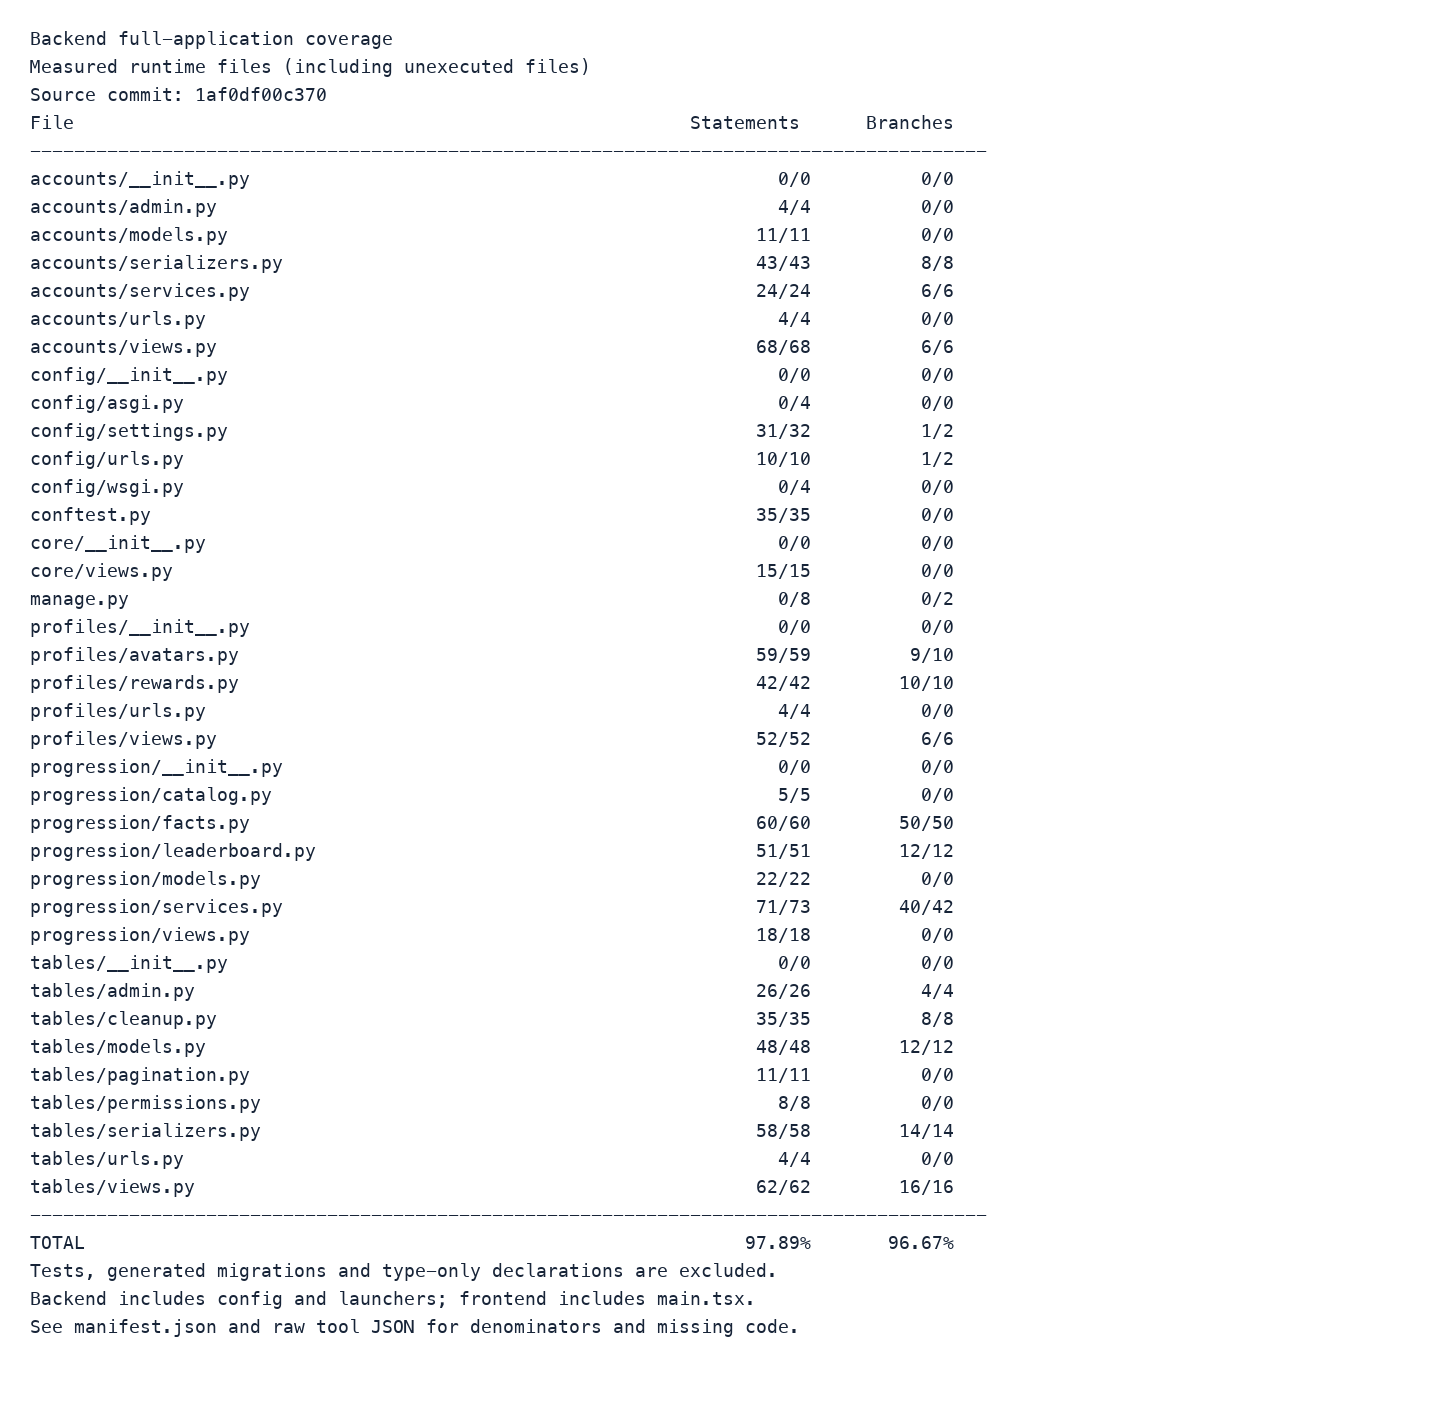
\includegraphics[width=\textwidth,height=.83\textheight,keepaspectratio]{../quality/evidence/backend-coverage.png}
\caption{Full backend per-file coverage generated from the tool's raw JSON.}\end{figure}
\begin{figure}[p]\centering
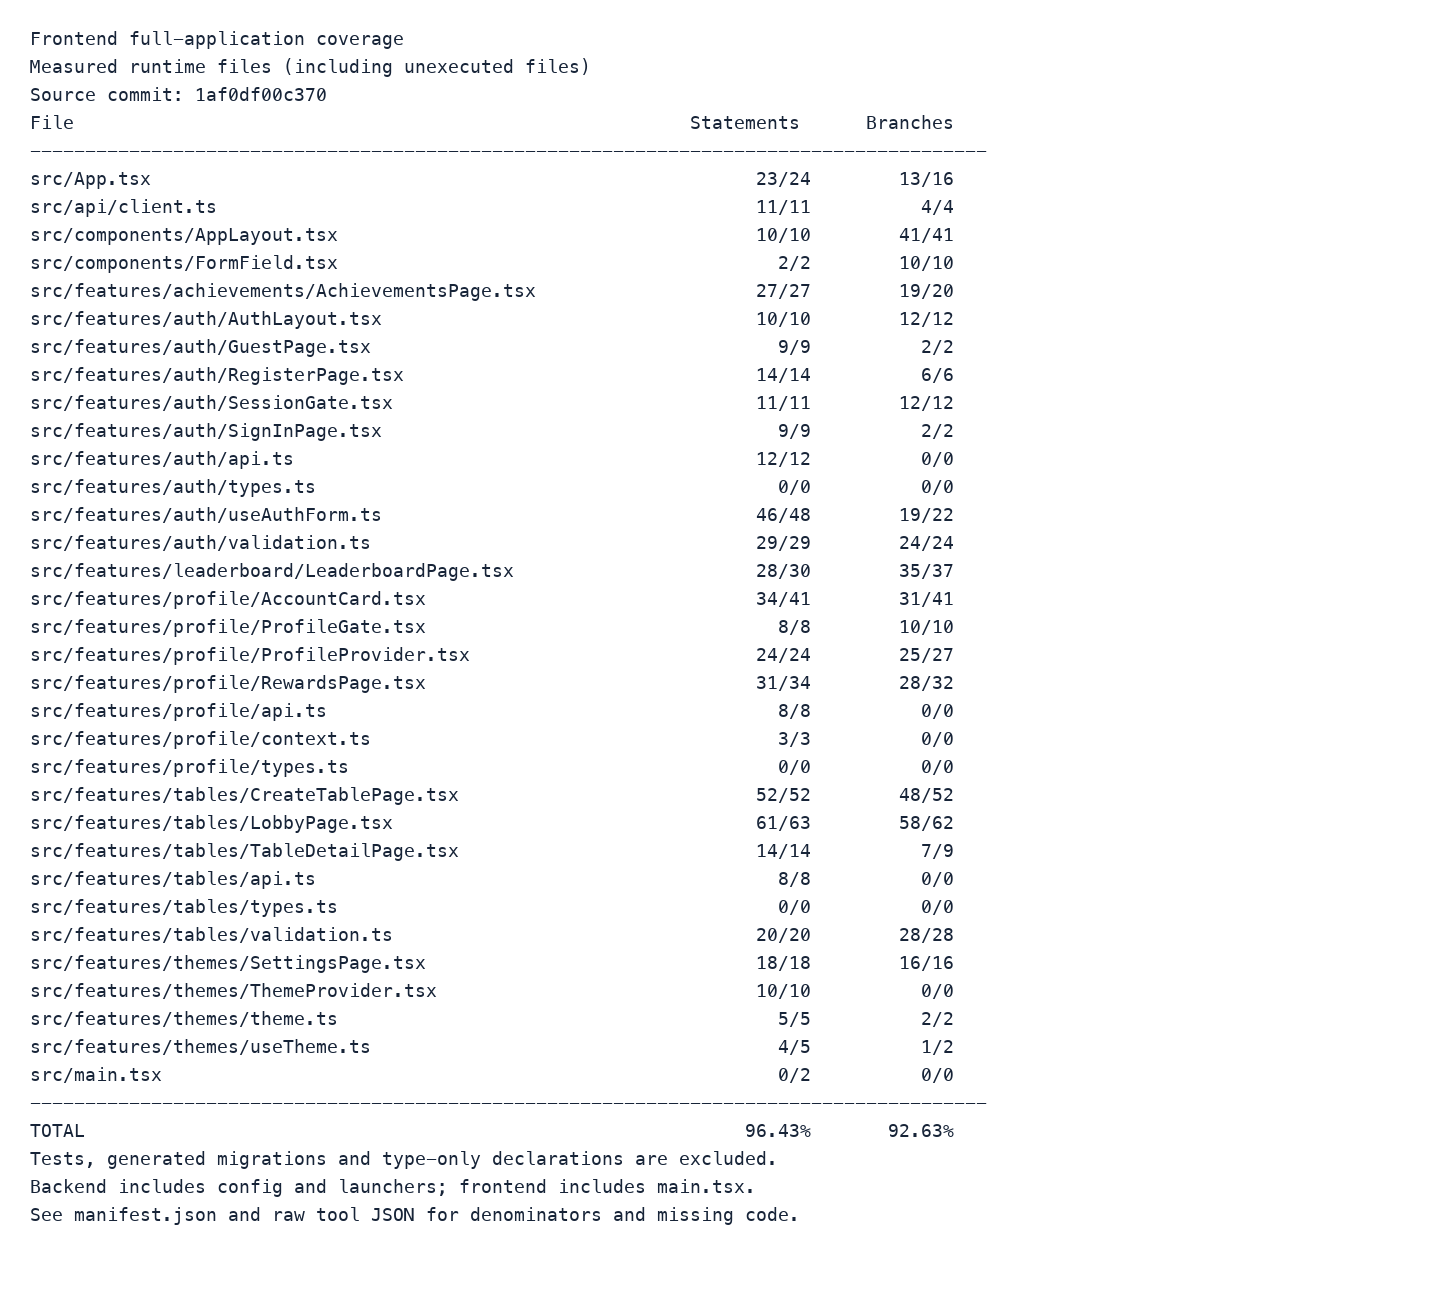
\includegraphics[width=\textwidth,height=.83\textheight,keepaspectratio]{../quality/evidence/frontend-coverage.png}
\caption{Full frontend per-file coverage generated from the tool's raw JSON.}\end{figure}
\clearpage

\subsection{Adequacy, gaps and improvement}
The test suite checks persistence, validation, CSRF, permissions, owner isolation, atomic failure/rollback, image content and cleanup, exact UTC claim boundaries, concurrent payouts, event retries and ranking ties/page boundaries. Frontend tests cover loading, retry, stale responses, invalid inputs and theme changes. Real-browser checks exercise actual registration, table/avatar/theme XP and ledger ranking in both themes and mobile/desktop layouts.

High coverage is useful regression evidence, not acceptance or feature completeness. Missing game, tournament and social integrations still need real end-to-end tests once their authoritative services exist. CLI bootstrap code may remain uncovered. Read the missing-line/branch lists rather than increasing a percentage through trivial mirrored tests. CI repeats full-scope checks and fails if either side does not exceed 80\% statement and 50\% branch coverage; reports remain truthful on failure.

\section{Process, Traceability and Retrospective}
The live Kanban Status options are Backlog, Ready, In progress, In review, Acceptance Test and Done. Acceptance Test was added immediately before Done while preserving all 39 existing statuses. Only professor/CTO acceptance authorizes Done. New commits reference actual issues \#45 and \#32; older hashes are mapped without rewriting original authorship.

Velocity is the accepted story-point total during the iteration. Cycle time uses actual In Progress and Acceptance Test timestamps under the team's convention. Neither metric can be reconstructed reliably from commit timestamps or newly corrected statuses; unknowns remain pending. The work log captures future actual records. Main delivery, peer review, submission timing and demo attendance are human/team responsibilities distinct from a local test run.

Proposed next-iteration improvements: verify the coverage scope before release; keep the planning/execution report current; record time and transitions when they occur; review small issue-linked commits; rehearse happy and failure paths with real data; disclose partial integrations early; and coordinate a backup presenter/recording without replacing required live attendance. Each teammate should add their own reflection rather than accepting generated prose as a personal statement.

\section{Release and Demo Checklist}
\begin{enumerate}\setlength{\itemsep}{1pt}\setlength{\parsep}{0pt}
\item Compare the reported October 27, 7:47 PM email time against the assignment release date; enter actual hours and confirm Moodle/demo dates.
\item Push original feature branches; peer-review and integrate without losing authorship. Main must contain the release before cutoff.
\item Run the full quality script, export truthful evidence for the source SHA, build this report and commit the PDF/source/images.
\item Rehearse S32/S18 real actions and failure cases. Show the proposed gameplay model separately from running features.
\item Every member presents their own work and can explain scope, tests and commits. Communicate a real absence in advance.
\item Record CTO decisions after the demo; accepted stories may move to Done and rejected work returns to Backlog.
\end{enumerate}


\clearpage
\appendix
\section{Actual work hours worksheet}
Enter actual hours, or honest retrospective estimates explicitly labelled as estimates, for each story. These are editable placeholders, not invented records. Confirm each contributor's work with that person; planned ownership and later repair work are distinct.

\begin{tabularx}{\textwidth}{@{}l l l X l@{}}
\toprule Iteration & Story & Planned owner & Contributor evidence & Actual hours\\\midrule
1 & S13 & Chris & Chris & TBD\\
1 & S10 & Chris & Chris & TBD\\
1 & S2 & Finn & Finn & TBD\\
1 & S1 & Finn & Finn & TBD\\
1 & S4 & Finn & Finn & TBD\\
1 & S23 & Kelechi & Kelechi & TBD\\
1 & S35 & Kelechi & Kelechi & TBD\\
1 & S5 & Royal & Chris's later repair; confirm original work & TBD\\
1 & S14 & Royal & Chris's later repair; confirm original work & TBD\\
1 & S29 & Royal & Chris's later repair; confirm original work & TBD\\\midrule
2 & S32 & Chris & Chris & TBD\\
2 & S18 & Chris & Chris & TBD\\
2 & S19 & Finn & Finn's feature branch & TBD\\
2 & S16 & Kelechi & Confirm with Kelechi & TBD\\
2 & S15 & Kelechi & Confirm with Kelechi & TBD\\
2 & S17 & Kelechi & Confirm with Kelechi & TBD\\
2 & S11 & Royal & Confirm with Royal & TBD\\
2 & S27 & Royal & Confirm with Royal & TBD\\
2 & S26 & Royal & Confirm with Royal & TBD\\\bottomrule
\end{tabularx}

Do not total unknown values as zero. Update the execution narrative and the CSV work log after the real values are supplied. Instructor-accepted points and cycle time require their own records.

\end{document}
